\chapter{Empirical Validation}
\label{chap:case-study}

The thesis now focuses on the application of the implemented features and methods in a real-world scenario. The goal is to demonstrate the practical applicability of the developed concepts and to validate the theoretical findings presented in the previous chapters.

\section{Physical Entity: Internet of Things Factory}
\label{sec:factory}
The framework has been applied on the Internet of Things-Factory (IOT) in Gütersloh, Germany \autocite{IoTFactory2024}. It is a cyber-physical system (CPS) \autocite{baheti2011cyber} mimicking industry-relevant processes in a smaller scale for research students. It consists of several stations that are partly interconnected via an assembly line or a delivery service conducted by automatic guided vehicles (AGVs). The factory is modular, so processes can be discovered module-wise in isolation. All modules are working on edge but are connected to a cluster that controls them. Theoretically, some stations can perform jobs of others. The main process also evaluated here is circular, meaning that the product is assembled and can be disassembled in a loop. The factory is shown in Figure \ref{fig:iotoverview}.

\begin{figure}[htbp]
  \centering
  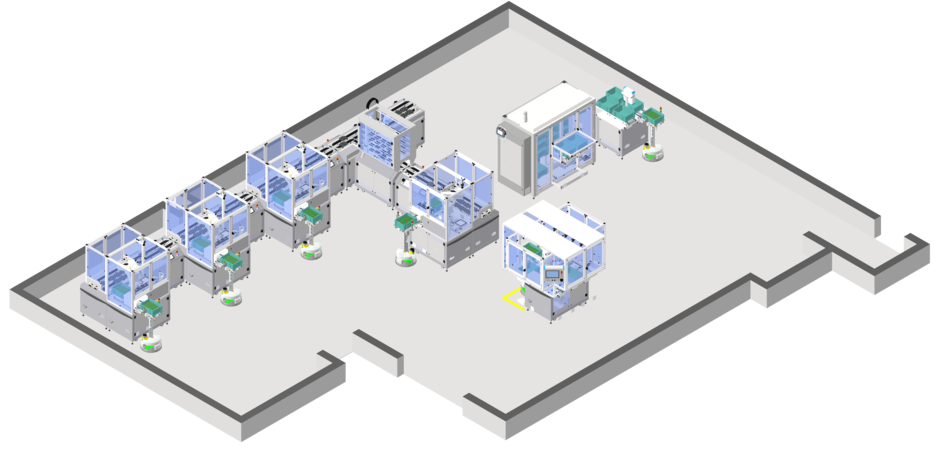
\includegraphics[width=0.7\textwidth]{figures/iot1.png}
  \caption[IoT Factory Overview]{Overview of the IOT factory. It consists of three production stations from left to right, which are followed by a sorting station and a packaging station. The stations are interconnected by an assembly line. Isolated from the assembly part, two AGVs are used to transport parts between the warehouse station (upper right) and another flexible workstation (right).}
  \label{fig:iotoverview}
  \caption*{Source: \autocite{IoTFactory2024}}
\end{figure}

The robot cells are responsible for performing transformation operations like assembling additional parts or testing functions.

\begin{figure}[htbp]
  \centering
  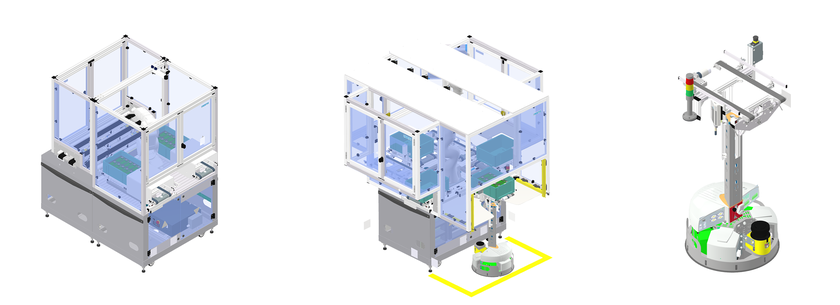
\includegraphics[width=0.8\textwidth]{figures/robots.png}
  \caption[Robot cells]{Two robot cells. The first cell is the main actor in this exemplary production process. Cell two is not part of the observed process here. The third image shows an AGV which transports boxes with assembled and disassembled parts to the stations.}
  \label{fig:robots}
  \caption*{Source: \autocite{IoTFactory2024}}
\end{figure}

The factory produces an exemplary product, consisting of a back part, a breadboard for several parts and a front panel. The parts to put on the breadboard are a display, gyroscope, an analog board and a weather station.

\begin{figure}[htbp]
  \centering
  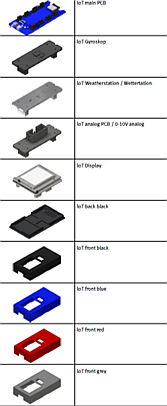
\includegraphics[width=0.2\textwidth]{figures/parts.png}
  \caption[Part variants]{The product consists of a back part, a breadboard and a front panel. The breadboard is used to put on several parts, such as a display, gyroscope, analog board and a weather station.}
  \label{fig:iotproduct}
  \caption*{Source: \autocite{IoTFactory2024}}
\end{figure}

The only colour produced at the moment is black. Not all parts can be put on the breadboard and there are several parts which conflict in size and location on the breadboard. Back and front cover are necessary parts and are assembled every time. The main part \texttt{main\_pcb} is also obligatory. It is placed at the beginning. Following that, the display or gyroscope can be assembled. If the display has been chosen, only the analog board or the weather station can be assembled. The weather station takes too much space on the breadboard for the gyroscope to be placed. If the analog board has been placed, the gyroscope is of course possible. The product is finished by placing the front cover and delivering the product to the sink.During the production, the factory gathers data via sensors. The data is saved in a database and can be used for further analysis. The database is relational and supports SQL queries.

Finally, the sequential order of the production process is as follows:

\begin{figure}[H]
  \centering
  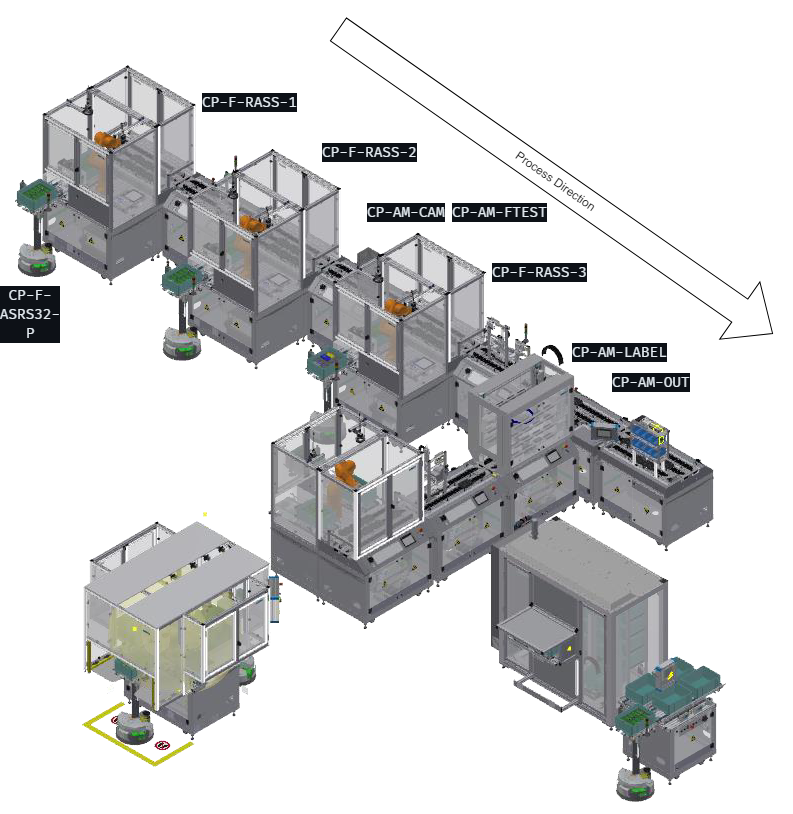
\includegraphics[width=0.7\textwidth]{figures/processdirection.png}
  \caption[Production process]{The blueprint with transitions between resources.}
  \label{fig:transitions}
  \caption*{Source: \autocite{IoTFactory2024}}
\end{figure}

\subsection*{Factory Dataset}

The dataset has been gathered from the database of the IoT Factory. In the code it is referred to as \texttt{real\_data}.

The dataset contains 18057 rows and 4696 orders from a time span of 22.04.2020 to 14.05.2024. There are no duplicate rows. Each row describes a unique operation step in an order. Roughly 40 percent of the rows contain missing values, which have been filled with zeros. The data has been mined from a MariaDB SQL database of the IoT Factory. Several tables have been aggregated to form the dataset. Without additional tables, no information about workplans, resources and operation numbers would be available. The dataset is filtered for promising trajectories of meaningful and intact process executions. The filter considers data between the 20.04.2020 and 22.04.2022, 02.05.2022 and 19.07.2022, 02.11.2022, 11.11.2022, 23.01.2022 and March 2023, each data inclusively.

The dataset contains the following columns:

\begin{itemize}
  \item \textbf{WPNo}: The workplan number of the specific workplan.
  \item \textbf{StepNo}: The step number of the specific workplan. The workplan is divided in sequential steps enumerated by this number.
  \item \textbf{ONo}: The order number of the specific order. Each order has a unique number.
  \item \textbf{OPos}: The order position of the specific order. The order position is the position of the order in the workplan.
  \item \textbf{Description}: The description of the specific step in spoken language.
  \item \textbf{OpNo}: The operation number of the specific operation. Each operation has a unique number.
  \item \textbf{NextStepNo}: The next step number of the specific step. This is the step that follows the current step.
  \item \textbf{FirstStep}: The first step of the specific workplan.
  \item \textbf{ErrorStepNo}: The error step number of the specific step. This is the step that is executed in case of an error.
  \item \textbf{Start}: The start time of the specific step.
  \item \textbf{End}: The end time of the specific step.
  \item \textbf{OPNoType}: The operation number type of the specific operation.
  \item \textbf{ResourceID}: The resource ID of the specific resource.
  \item \textbf{ErrorStep}: Is this step an error step (yes/no)?
  \item \textbf{ErrorRetVal}: The error return value of the specific step.
  \item \textbf{Active}: Is this step active (yes/no)?
  \item \textbf{op\_desc}: The operation description of the specific operation, which is more specific than the description.
  \item \textbf{ResourceName}: The name of the specific resource.
  \item \textbf{resource\_desc}: The description of the specific resource.
  \item \textbf{workplan\_desc}: The description of the specific workplan.
  \item \textbf{workplantype\_desc}: The description of the specific workplan type.
  \item \textbf{case\_id}: The case ID of the specific case.
  \item \textbf{Description\_Encoded}: The description of the specific step ordinally encoded.
\end{itemize}

The operations performed can be seen in the following:

\begin{enumerate}
  \item \textbf{Release a part on stopper 1}: The AGV delivered the box with the parts to be manufactured to the first station. The box is travelling over the assembly line to the first station where the first part is released.
  \item \textbf{Place cover to assembly place}: The first part is placed on the assembly place. The cover is placed on top of the part as the first piece of the product.
  \item \textbf{Assemble part from box on RASS1 - MAIN PCB}: The main PCB is assembled on the cover. This is the first configured part of the product. The main PCB is the breadboard of the product.
  \item \textbf{Switch on PCB}: The main PCB is switched on. This is necessary to activate it.
  \item \textbf{Assemble part from box on RASS1 - DISPLAY}: The display is assembled on the main PCB. This is the second configured part of the product. The display is one optional part of the product. This factors out one product variant.
  \item \textbf{Move part to pallet on belt}: The product is moved to the pallet on the belt for further processing.
  \item \textbf{Measure a part (analog)}: The product is measured. This is necessary to ensure the quality of the product for later steps.
  \item \textbf{Assemble part from box on RASS2 - ANALOG}: The analog part is assembled on the product. This is the third configured part of the product. The analog part is also one optional part of the product.
  \item \textbf{Assemble part from box on RASS2 - GYROSCOPE}: The gyroscope is assembled on the product. This is the fourth configured part of the product. The gyroscope is also one optional part of the product.
  \item \textbf{Move part to pallet on belt}: The product is moved to the pallet on the belt for further processing.
  \item \textbf{Check analog}: The analog part is checked. This is necessary to ensure the quality of the product for later steps.
  \item \textbf{Check gyroscope}: The gyroscope is checked. This is necessary to ensure the quality of the product for later steps
  \item \textbf{Assemble part from box on RASS3 - FRONT COVER}: The front cover is assembled on the product. This is the last configured part of the product. The front cover is the last part of the product.
  \item \textbf{Move part to pallet on belt}: The product is moved to the pallet on the belt for further processing.
  \item \textbf{Test connection to IoT main PCB}: The connection to the IoT main PCB is tested. This is necessary to ensure the quality of the product for later steps.
  \item \textbf{Test the function of the touch display}: The touch display is tested. This is necessary to ensure the quality of the product for later steps.
  \item \textbf{Test the analog input/output shield}: Analog PCB is tested.
  \item \textbf{Test the historical gyroscope data}: The gyroscope is tested.
  \item \textbf{Print Label}: The label is printed. The label contains information about the product configuration, the time manufactured and the serial number.
  \item \textbf{Deliver Part}: The final product is delivered to the sink.
\end{enumerate}

Per step, several resources are involved. The following table shows the utilized resources per step:

\begin{table}[H]
  \centering
  \footnotesize
  \caption[Production steps and resources]{Steps and Resources Used}
  \label{tab:description-resources}
  \begin{tabular}{@{}p{0.4\textwidth}p{0.4\textwidth}@{}}
    \toprule
    \textbf{Process Step Name}                    & \textbf{Resource Name}                \\
    \midrule
    Release a part on stopper 1                   & CP-F-ASRS32-P                         \\
    Place cover to assembly place                 & CP-F-RASS-1, CP-F-RASS-2, CP-F-RASS-3 \\
    Assemble part from box on RASS1 - MAIN PCB    & CP-F-RASS-1                           \\
    Switch on PCB                                 & CP-F-RASS-1                           \\
    Assemble part from box on RASS1 - DISPLAY     & CP-F-RASS-1                           \\
    Move part to pallet on belt                   & CP-F-RASS-1, CP-F-RASS-2, CP-F-RASS-3 \\
    Measure a part (analog)                       & CP-AM-MEASURE                         \\
    Assemble part from box on RASS2 - ANALOG      & CP-F-RASS-2                           \\
    Assemble part from box on RASS2 - GYROSCOPE   & CP-F-RASS-2                           \\
    Move part to pallet on belt                   & CP-F-RASS-1, CP-F-RASS-2, CP-F-RASS-3 \\
    Check analog                                  & CP-AM-CAM                             \\
    Check gyroscope                               &                                       \\
    Assemble part from box on RASS3 - FRONT COVER & CP-F-RASS-3                           \\
    Move part to pallet on belt                   & CP-F-RASS-1, CP-F-RASS-2, CP-F-RASS-3 \\
    Test connection to IoT main PCB               & CP-AM-FTEST                           \\
    Test the function of the touch display        & CP-AM-FTEST                           \\
    Test the analog input/output shield           & CP-AM-FTEST                           \\
    Test the historical gyroscope data            & CP-AM-FTEST                           \\
    Print Label                                   & CP-AM-LABEL                           \\
    Deliver Part                                  & CP-AM-OUT                             \\
    \bottomrule
  \end{tabular}
  \caption*{Source: \Textcite{IoTFactory2024}}
\end{table}


This process has been identified as the ground-truth process. The process is circular, meaning that the product is assembled and can be disassembled in a loop. The process is also modular, so that the product can be assembled in different configurations. The process is also flexible, the product can be assembled in different ways.

\section{Digital Entity: Open Factory Twin}
\label{sec:automated-digital-twin}

The Simulation-Based Digital Twin (SBDT) for the IoT Factory use case was developed using the Open Factory Twin (OFacT) framework \autocite{ofact-intern}. OFacT is an open-source digital twin framework specifically designed for modelling, simulating, and controlling production and logistics environments. Its goal is to support system design, planning, and operational control during the entire lifecycle of such systems.

A principle of OFacT is the separation between the static description of the system and its dynamic behaviour. This is achieved by distinguishing between:

\begin{itemize}
  \item \textbf{State Model:} This component represents the static structure of the factory, its components (resources, parts, layout), their properties, relationships, and the potential processes or behaviours they can exhibit.
  \item \textbf{Agent Control:} This component implements the dynamic logic that controls the systems operation during simulation, making decisions about resource allocation, process execution sequences, and handling events based on the state model.
\end{itemize}

The construction of the State Model within OFacT uses structured input methods, such as Excel files, where different sheets correspond to specific classes within the OFacT metamodel, inspired by \textcite{schwede2024learning}. To model the IoT Factory scenario (\autoref{sec:factory}), the relevant components of the OFacT State Model were defined, including:

\begin{itemize}
  \item \textbf{Plant}: The overall entity of production. The plant name used here was \texttt{iot\_factory}.
  \item \textbf{EntityType}: All entities have to be defined here. This ranges from the parts, resources and AGVs to the factory itself.
  \item \textbf{StationaryResource}: Stationary resources are static and can not move. In this case, these are the RASS stations, measurement-, cam-, function test- and labelling station. The AGVs are not stationary resources, because they can move.
  \item \textbf{Storage}: Storage units contain parts. They are used to traverse the parts through the factory. In this context, the warehouse and box storage, have been modelled.
  \item \textbf{Warehouse}: This is a static storage unit where the parts are stored in boxes until they are processed.
  \item \textbf{WorkStation}: Workstations are resources which perform processes on parts. In our use case, these are the RASS stations.
  \item \textbf{ConveyorBelt}: There is one belt where the storage units traverse through the factory.
  \item \textbf{NonStationaryResource}: There are no non-stationary resources.
  \item \textbf{PassiveMovingResource}: One artificial passive moving resource has been mod
  \item \textbf{Process}: Contains processes and value added processes (VAP). VAP are adding features to parts and modify it. For each activity in the data a VAP has been created.
  \item \textbf{ProcessController}: This controller summarizes all processes to come and connects them.
  \item \textbf{ResourceModel}: Resource groups are formulated for activities like montage, identifying to attach the relevant parts to these resources. This way, main resources and parts are getting matched.
  \item \textbf{ProcessTimeModel}: Each part receives a time simple time distribution to account for its production time.
  \item \textbf{QualityModel}: Each part receives a bernoulli distribution to account for its quality. In the dataset, no quality information existed.
  \item \textbf{TransitionModel}: This model connects possible origins to possible destinations, to that the traversal of the parts can be modelled correctly. The packaging has been modelled as transition model.
  \item \textbf{TransformationModel}: This model contains an artificial transformation model.
  \item \textbf{Time}: Process execution plans get a starting time here.
  \item \textbf{Part}: Parts are connected to their EntityType here. There is also information attached where the part is stored or situated in.
  \item \textbf{Sales}: Lists the features and feature cluster. This matches the building rules. Parts have to be defined as features here.
  \item \textbf{CustomerGeneration}: Customer generation logic.
  \item \textbf{Customer}: List of customers.
  \item \textbf{Orders}: The orders with their requested features.
  \item \textbf{Process}: Contains processes and value added processes (VAP). VAP are adding features to parts and modify it. For each activity in the data a VAP has been created.
  \item \textbf{TransitionModel}: This model connects possible origins to possible destinations, to that the traversal of the parts can be modelled correctly. The packaging has been modelled as transition model.
  \item \textbf{TransformationModel}: This model contains an artificial transformation model.
\end{itemize}

By defining these elements according to the IoT Factory characteristics, a detailed static model was created within the OFacT framework. For simulation purposes, the state model then gets played out \autoref{fig:playinoutreplay} with orders. The orders contain this model then served as the basis for running simulations to generate process execution data, forming the SBDT dataset used in this thesis for comparison against real-world data.

\subsection*{SBDT Dataset}

The dataset gathered from the SBDT is referred to as \texttt{sim\_data}. The OpenFactoryTwin provides a method to deserialize the simulated orders and save them in a CSV file. The dataset then gets converted to the OCEL structure. For this endeavour, a separate connector logic has to be implemented in every use case.\footnote{See \texttt{src/connector/ofact} for the connector here.}

The connector's output follows a standardized structure defined by the \texttt{OutputStructure} class, which ensures consistency across different data sources. The connector first deserializes the dynamic state model from a pickle file, accessing the full simulation state. Only actual process executions (not planned ones) are kept for further processing, identified by the `ACTUAL' flag in their event type. The connector creates mapping dictionaries for various categorical attributes following the OCED standard. The categories can be defined by the modeller beforehand, which is the case here. The IDs are based on enumeration and default to -1 if the category has not been found in the list:

\begin{itemize}
  \item \textbf{Part ID Mapping:} Uses domain expertise to identify part types from process names, normalizing text (lowercase, no whitespace) to match against a predefined list of possible parts. This list contains possible parts from \autoref{fig:iotproduct}.
  \item \textbf{Process Type Categorization:} Assigns process steps to expert-defined categories such as `machine,' `feature,' `endproduct,' `test,' and `transport' based on keywords in process names. These types have been assigned by the modeller and are of free choice.
  \item \textbf{Process ID Mapping:} Creates unique integer identifiers for each distinct process description based on enumeration.
  \item \textbf{Resource ID Mapping:} Generates unique identifiers for each resource involved in the process executions based on enumeration.
  \item \textbf{Temporal Data Extraction:} The connector extracts start and end times for each process execution.
\end{itemize}

Process executions are associated with their respective order IDs, establishing the connection between individual process steps and the orders they belong to. All extracted information is then consolidated into a standardized DataFrame structure with properly typed columns as defined in the \texttt{OutputStructure} class. The connector also includes a validation step to ensure that the generated DataFrame adheres to the expected structure and data types, raising an error if any discrepancies are found.

A key aspect of the connector's functionality is the non-mandatory integration of domain knowledge into the data transformation process. Instead of relying only on the raw data structure, the connector employs expert-defined categorizations and normalization procedures to ensure semantic consistency in the transformed data.

For example, the part identification logic uses a predefined list of potential parts (such as `GYROSCOPE,' ``MAIN PCB,' ``FRONT COVER,' etc.) and searches for these terms within process descriptions. Similarly, the process type categorization uses domain-specific groupings like `machine,' `feature,' and `test' based on keywords found in process names. The \texttt{sim\_data} rows will receive the label $0$ for \texttt{is\_valid}, because the black-box model should learn to distinguish between real and simulated data to perform VVUQ. The entries of the \texttt{real\_data} receive $1$ for \texttt{is\_valid}.


\section{Data Pipeline}
\label{sec:data-pipeline}

Several preprocessing steps had to be performed to account for the fact that the SBDT simulated only one variant of the product: 'analog', 'cover', 'display', 'gyroscope', 'pcb' and the involved machines. This yielded the necessity to make both datasets congruent to each other. The following steps were performed:

\begin{itemize}
  \item The \texttt{sim\_data} dataset was aligned for the same time period as the \texttt{real\_data} dataset. The SBDT chose the time of order as the production time. In the modelling phase, when adaptive feature selection had been performed to identify if the SBDT was able to learn the Time Model, only \textit{relative} time features like duration were chosen which were developed in \autoref{sec:feature-engineering}.
  \item The \texttt{real\_data} dataset was filtered for the same process steps as the \texttt{sim\_data} dataset. This means that only the process steps which are present in the \texttt{sim\_data} dataset were kept, producing only one product variant. This has also been applied on the part\_id, the process\_type and resource\_id columns. The IDs based on enumeration had to be mapped to the original IDs in \texttt{real\_data} to ensure that the correct IDs are used in the simulation. The mapping was done through the JSON files generated by the connector.
  \item Both datasets have been cleaned and entries containing invalid IDs were removed. This means that all entries which are not present in the mapping dictionaries were removed. The mapping dictionaries are generated by the connector and contain only valid IDs per definition.
  \item Only a subset of all performed processes was included (in detail, all \texttt{process\_id} $\le 26$). These processes all have the \texttt{process\_type} 'machine', 'feature' or 'endproduct'. The processes with the \texttt{process\_type} 'test' and 'transport' were removed. This was done to ensure that only the relevant processes are included in the dataset.
\end{itemize}

This cleaning step was not corrupting the data to facilitate easier learning of the models, it removed epistemic uncertainty. For example, some rows contained invalid names.
The \texttt{real\_data} dataset was then concatenated with the \texttt{sim\_data} dataset. The concatenation was done by appending the \texttt{sim\_data} dataset to the \texttt{real\_data} dataset. The resulting dataset contains all process steps from both datasets. The resulting dataset is referred to as \texttt{final\_data}. The unification before concatenation was necessary to ensure that no logical flaws are present in the data.

The \texttt{final\_data} dataset after preprocessing as described contains 1978 rows and 56 orders with 24 features. The following section elaborates how these features were generated.

\subsection*{Feature Engineering}
\label{sec:feature-engineering}

Several features have been engineered to assist both the whitebox and blackbox model on the validation task. The features were furher introduced to empower adaptive feature selection (AFS) regarding the model components of the SBDT \autocite{schwede2024learning}. This way, if the features sufficiently explain the data, the conclusion can be made that the SBDT was able to learn the respective model component.

The following features were generated with domain knowledge:

\begin{itemize}
  \item \textbf{KPIs}: Throughput, setup time, lead time and cycle time have been added to assist the VVUQ, see \autoref{sec:relevant-kpis}. They allow PPC VVUQ to be performed. They further can be integrated to check if the Time Model has been learned.
  \item \textbf{duration}: The duration of the process step. This feature is important to understand how long the process step took. It is calculated as the difference between the start and end time of the process step.
  \item \textbf{sequence\_number}: The sequence number of the process step. This feature is important to understand the order of the process steps. It is calculated by grouping the data by the process execution ID and then enumerating the process steps within each group based on the end time. This way, the sequence number enumerates each process step per order. It helps the \texttt{DecisionTreeClassifier} to learn the order of the process steps.
  \item \textbf{is\_not\_weekday}: A binary feature indicating whether the process step occurred on a weekend (1) or a weekday (0). No activities have been performed on weekends in the factory, so weekend activity is an anomaly.
  \item \textbf{is\_break}: A binary feature indicating whether the process step occurred during a break (1) or not (0). No activities have been performed during breaks in the factory, so break activity is an anomaly as well.
  \item \textbf{hour\_of\_day}: The hour of the day when the process step occurred. This feature is important to understand the time of day when the process step took place. It is calculated as the hour of the start time of the process step.
  \item \textbf{day\_of\_week}: The day of the week when the process step occurred. It is also calculated as the day of the week of the start time of the process step.
  \item \textbf{day\_of\_week\_sin and day\_of\_week\_cos}: A periodic time feature representing the sine and cosine of the day of the week, which helps capture weekly patterns in the data.
  \item \textbf{hour\_of\_day\_cos and hour\_of\_day\_sin}: A periodic time feature representing the cosine and sine of the hour of the day, which helps capture daily patterns in the data.
\end{itemize}

Days and hours are cyclical features that require special handling. Representing them as raw integers fails to capture their continuity (e.g., hour 23 is close to hour 0). To address this, the feature $x$ with period $P$ using sine and cosine functions has been transformed, effectively mapping it onto a unit circle:
\begin{equation}
  x_{\sin} = \sin\left(\frac{2 \pi x}{P}\right) \quad ; \quad
  x_{\cos} = \cos\left(\frac{2 \pi x}{P}\right)
  \label{eq:sincos_transform}
\end{equation}
This provides a continuous, two-dimensional representation $(x_{\cos}, x_{\sin})$ that preserves the cyclical nearness of values.

In this work, this transformation is applied to:

\begin{itemize}
  \item \textbf{Hour of Day (`hour\_of\_day`):} $P=24$. Features: $\text{hour\_of\_day}_{\sin}$, $\text{hour\_of\_day}_{\cos}$.
  \item \textbf{Day of Week (`day\_of\_week`):} $P=7$. Features: $\text{day\_of\_week}_{\sin}$, $\text{day\_of\_week}_{\cos}$.
\end{itemize}

Figure \ref{fig:time-encoding} illustrates this concept for the hour of the day. This encoding helps machine learning models better understand and utilize the cyclical nature of time.

\section{Validation Methodology and Setup}
With the integration of these features, AFS can be performed. For the statistical soundness of the analysis, a permutation test will be performed to assess the significance of the results. The following sections outline the testing procedure and the specific components of the SBDT that will be evaluated.

\subsection*{Permutation Testing for Statistical Significance}
\label{sec:model-logic}

As laid out in the methodology chapter \autoref{sec:permtest}, a permutation test will be conducted.

\noindent The null hypothesis ($H_0$) claims that the SBDT accurately represents the real system with respect to the features $\mathcal{F}_c$, meaning the data distributions are indistinguishable:
\begin{equation}
  H_0: \mathcal{D}_{real}(\mathbf{X} | \mathcal{F}_c) = \mathcal{D}_{sim}(\mathbf{X} | \mathcal{F}_c)
  \label{eq:h0}
\end{equation}

\noindent The alternative hypothesis ($H_1$) claims that the SBDT does \textit{not} accurately represent the real system, and the distributions are statistically distinguishable using the features $\mathcal{F}_c$:
\begin{equation}
  H_1: \mathcal{D}_{real}(\mathbf{X} | \mathcal{F}_c) \neq \mathcal{D}_{sim}(\mathbf{X} | \mathcal{F}_c)
  \label{eq:h1}
\end{equation}

\noindent Under this framework, if a classifier trained on the feature set $\mathcal{F}_c$ achieves performance significantly better than chance at distinguishing between real ($y=1$) and simulated ($y=0$) data, it provides evidence to reject $H_0$ in favour of $H_1$. This would imply that the SBDT component $c$ has \textit{not} been learned accurately, as detectable discrepancies exist. Conversely, if the classifier performs poorly (close to random chance), it fails to reject $H_0$, suggesting that, based on the features $\mathcal{F}_c$, the simulated data is consistent with the real data for that component.

\subsection*{Testing the SBDT Components}
To rigorously evaluate the SBDTs fidelity concerning different process aspects, the thesis implements the hypothesis testing framework outlined previously (testing $H_0$: \autoref{eq:h0} against $H_1$: \autoref{eq:h1}). This involved using machine learning classifiers to determine if statistically significant differences exist between the real process data ($\mathcal{D}_{real}$, labelled $y=1$) and the simulated data ($\mathcal{D}_{sim}$, labelled $y=0$) based on specific feature subsets ($\mathcal{F}_c$) corresponding to key SBDT model components.

The analysis was performed separately for distinct feature subsets $\mathcal{F}_c$, each clustered to reflect the behavior exhibited by specific SBDT components. Based on the feature engineering described in \autoref{sec:feature-engineering}, several targeted feature sets were defined. The \texttt{time\_model} subset encompasses temporal patterns and cyclical time representations, including \texttt{duration}, \texttt{sequence\_number}, cyclical encodings (\texttt{hour\_of\_day\_cos}, \texttt{hour\_of\_day\_day\_sin}, \texttt{day\_of\_week\_cos}, \texttt{day\_of\_week\_sin}), and temporal status indicators (\texttt{is\_break}, \texttt{is\_not\_weekday}). For operational resource allocation, the \texttt{resource\_model} subset includes categorical identifiers (\texttt{resource\_id}, \texttt{part\_id}, \texttt{process\_id}). To capture product transformations, the \texttt{transformation\_model} subset contains \texttt{part\_id}, \texttt{process\_id}, and \texttt{sequence\_number}. Movement patterns are represented in the \texttt{transition\_model} subset through \texttt{part\_id}, \texttt{resource\_id}, \texttt{sequence\_number}, and \texttt{duration}. Process execution characteristics are encapsulated in the \texttt{process\_model} subset via \texttt{process\_id}, \texttt{duration}, and \texttt{sequence\_number}. Additionally, the \texttt{kpi\_based} subset includes performance indicators (\texttt{throughput}, \texttt{cycle\_time\_sec}, \texttt{lead\_time\_sec}, \texttt{setup\_time\_sec}). Finally, an \texttt{all\_features} set combined all available engineered features to provide a comprehensive perspective.

\subsection*{Permutation Testing Procedure}

The practical implementation of the test described in \autoref{eq:pvalue_perm} followed these steps for each feature subset $\mathcal{F}_c$:

\begin{algorithm}[H]
  \caption[Permutation Testing]{Multi-Run Permutation Testing}
  \label{alg:permutation_testing_symbolic}
  \begin{algorithmic}[1]
    \footnotesize % Font size
    % -----------

    \Require % Input:
    \Statex \hspace{\algorithmicindent} Concatenated Dataset $\mathcal{D}_{final}$ (Features $\mathbf{X}$, Labels $y \in \{0,1\}$),
    \Statex \hspace{\algorithmicindent} Feature Subsets for model components $\{\mathcal{F}_c\}_{c=1}^C$,
    \Statex \hspace{\algorithmicindent} Runs $n_{runs}$, Permutations $N$, Significance level $\alpha$, Model Type $M_{type}$ \Comment{DTree, BiLSTM}
    \Ensure % Output:
    \Statex \hspace{\algorithmicindent} Results $R : \{c \mapsto (\bar{S}_{obs}, \sigma_{S_{obs}}, \bar{p}, RR)\}$ \Comment{Map component to aggregated stats}
    \medskip

    \State $R := \emptyset$ \Comment{Initialize results map}
    \medskip

    \ForAll{feature subset $\mathcal{F}_c$ for component $c$}
    \State $S_{obs\_list} := [\,]$; $p_{list} := [\,]$ \Comment{Initialize arrays for run results}
    \medskip
    \For{$run = 1$ to $n_{runs}$}
    \State $seed \leftarrow \text{RandomSeed}()$
    \State $(\mathcal{D}_{train}, \mathcal{D}_{test}) \leftarrow \text{Split}(\mathcal{D}_{final}, \mathcal{F}_c, seed)$ \Comment{Split stratified on $y$}
    \State $M \leftarrow \text{Train}(M_{type}, \mathcal{D}_{train})$ \Comment{Train on $(\mathbf{X}_{train}, \mathbf{y}_{train})$ using features $\mathcal{F}_c$}
    \medskip

    \State $\hat{\mathbf{p}}_{test} \leftarrow M(\mathbf{X}_{test})$ \Comment{Predict $P(y=1|\mathbf{X}_{test})$ using trained model $M$}
    \State $S_{obs} \leftarrow \text{ROC\_AUC}(\mathbf{y}_{test}, \hat{\mathbf{p}}_{test})$ \Comment{Observed score}
    \medskip

    \State $S_{perm\_list} := [\,]$
    \For{$i = 1$ to $N$}
    \State $\mathbf{y}_{test, perm}^{(i)} \leftarrow \text{Permute}(\mathbf{y}_{test})$ \Comment{Randomly shuffle test labels}
    \State $S_{perm, i} \leftarrow \text{ROC\_AUC}(\mathbf{y}_{test, perm}^{(i)}, \hat{\mathbf{p}}_{test})$ \Comment{Score vs fixed $\hat{\mathbf{p}}_{test}$}
    \State Append $S_{perm, i}$ to $S_{perm\_list}$
    \EndFor
    \medskip

    \State $count_{ge} \leftarrow \sum_{i=1}^{N} \mathbb{I}(S_{perm\_list}[i] \ge S_{obs})$
    \State $p_{run} \leftarrow count_{ge} / N$ \Comment{p-value for this run}
    \medskip

    \State Append $S_{obs}$ to $S_{obs\_list}$; Append $p_{run}$ to $p_{list}$ \Comment{Store run results}
    \EndFor \Comment{End runs}
    \medskip

    \State $\bar{S}_{obs} \leftarrow \text{Mean}(S_{obs\_list} | \text{not NaN})$ \Comment{Calculate mean of valid observed scores}
    \State $\sigma_{S_{obs}} \leftarrow \text{StdDev}(S_{obs\_list} | \text{not NaN})$ \Comment{Calculate $\sigma$ of valid observed scores}
    \State $\bar{p} \leftarrow \text{Mean}(p_{list} | \text{not NaN})$ \Comment{Calculate mean of valid p-values}
    \State $RR \leftarrow \text{Mean}(\mathbb{I}(p < \alpha) \mid p \in p_{list}, p \neq \text{NaN})$ \Comment{Rejection Rate on valid p-values}
    \State $R[c] \leftarrow (\bar{S}_{obs}, \sigma_{S_{obs}}, \bar{p}, RR)$ \Comment{Store aggregated results for component $c$}
    \medskip
    \EndFor \Comment{End feature subsets}

    \State \Return $R$

  \end{algorithmic}
\end{algorithm}

\begin{enumerate}
  \item \textbf{Data Splitting:} The combined dataset (\texttt{final\_data}) was split into stratified training ($\mathcal{D}_{train}$) and testing ($\mathcal{D}_{test}$) sets, ensuring proportional representation of real ($y=1$) and simulated ($y=0$) data in both sets. A random seed was used for reproducibility within a single run.
  \item \textbf{Model Training:} The chosen classifier (DTree or BiLSTM) was trained on $\mathcal{D}_{train}$ using only the features in $\mathcal{F}_c$.
  \item \textbf{Observed Statistic Calculation:} The trained model was evaluated on the original test set $\mathcal{D}_{test}$. The performance metric, specifically the ROC AUC score \autoref{eq:auc}, was calculated and recorded as the observed statistic, $S_{obs}$.
  \item \textbf{Null Distribution Generation (Permutation):} To generate the null distribution, $N$ permutations were performed. Critically, an efficient approach was used, particularly for the computationally intensive BiLSTM model:
        \begin{itemize}
          \item The trained model generated predictions (binary $\hat{\mathbf{y}}_{test}$) and class probabilities (specifically for the positive class, $\hat{\mathbf{p}}_{test}$) on the original test set $\mathcal{D}_{test}$ \textit{once}.
          \item For each permutation $i=1...N$: The *true labels* $\mathbf{y}_{test}$ of the test set were randomly shuffled, creating $\mathbf{y}_{test, perm}^{(i)}$.
          \item The permuted statistic $S_{perm, i}$ was calculated by comparing the shuffled labels $\mathbf{y}_{test, perm}^{(i)}$ against the fixed probabilities $\hat{\mathbf{p}}_{test}$ (i.e., calculating ROC AUC between $\mathbf{y}_{test, perm}^{(i)}$ and $\hat{\mathbf{p}}_{test}$). This avoids retraining the model for each permutation. (A similar principle was applied for the Decision Tree, comparing permuted labels against fixed predictions/probabilities).
        \end{itemize}
  \item \textbf{P-value Calculation:} The p-value was computed as the proportion of permutation statistics greater than or equal to the observed statistic, following \autoref{eq:pvalue_perm}.
        \begin{equation}
          p = \frac{\sum_{i=1}^{N} \mathbb{I}(S_{perm, i} \ge S_{obs})}{N}
          \nonumber
        \end{equation}
\end{enumerate}

\section{Results and Interpretation}
The feature subsets are equal to the model components, as noted. The following UpSet plot summarizes the feature subsets used for the SBDT components.

\begin{figure}[htbp]
  \centering
  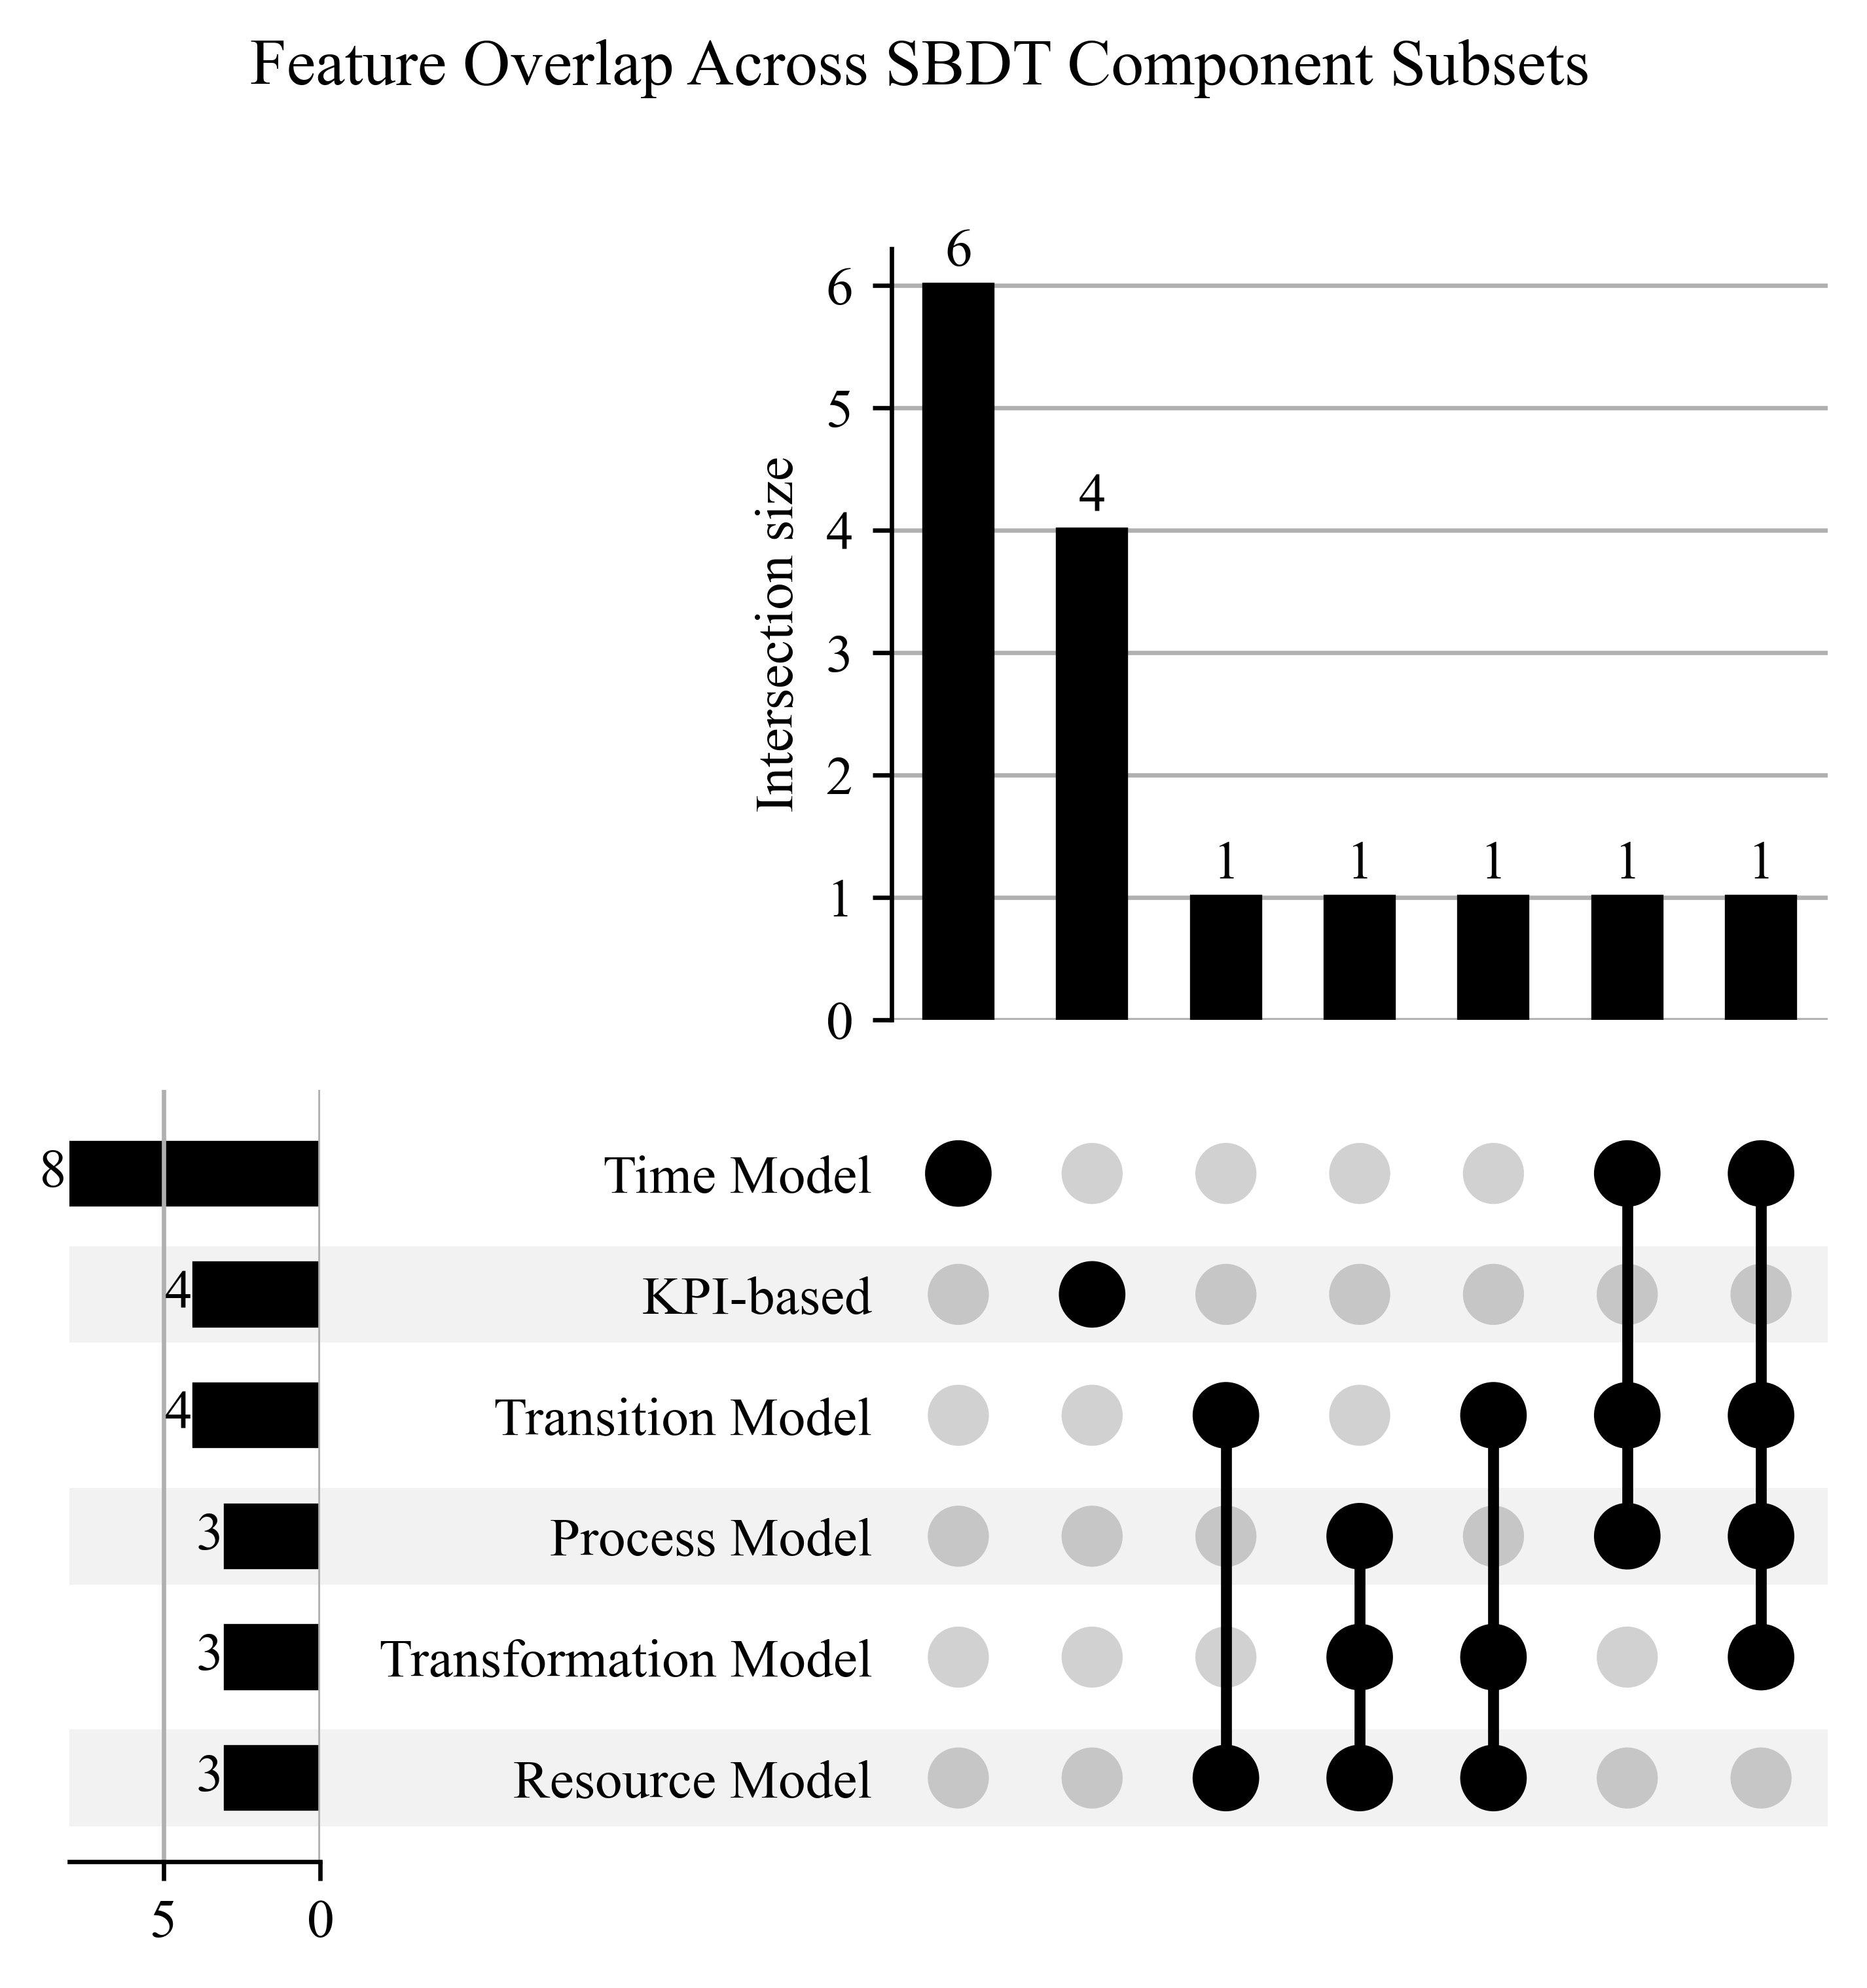
\includegraphics[width=0.7\textwidth]{figures/upset.png}
  \caption[UpSet plot]{UpSet plot visualizing feature overlap across categories. Left bars show total features per category; top bars show counts for specific intersections defined by the dot matrix below.}
  \caption*{Source: Own illustration.}
  \label{fig:upsetplot}
\end{figure}

The plot highlights that the time model has the largest number of unique features (6 features), consisting primarily of derived temporal sinusoidal and cosine encodings and status dummy variables. The KPI category also contains a distinct set of 4 unique features, representing specific performance metrics. These exclusive memberships indicate that temporal representation and performance indicators introduce the most diverse information into the overall feature space.
Several other features show significant overlap, signifying their role as core concepts linking multiple perspectives. Key identifiers like process\_id are shared across resource model, transformation model, and process model, while part\_id links resource model, transformation model, and transition model. The feature sequence\_number exhibits the highest degree of intersection among the detailed combinations, connecting time model, transformation model, transition model, and process model, underscoring its importance in relating temporal sequence to various operational views. Similarly, duration connects time model, transition model, and process model, and resource\_id connects resource model and transition model.

Based on the aggregated results, the fidelity of the SBDT component corresponding to the feature set $\mathcal{F}_c$ was assessed. A high \textit{rejection rate} $RR$ (e.g., consistently above 0.5 across the 10 runs) was interpreted as strong evidence against the null hypothesis $H_0$. This indicates that the classifier could reliably distinguish between real and simulated data based on the features $\mathcal{F}_c$, suggesting that the corresponding SBDT component was \textit{not learned accurately}. Conversely, a low rejection rate suggests insufficient evidence to reject $H_0$, implying the SBDT component might be \textit{adequately learned}, or at least its potential inaccuracies were not detectable by the classifier using the given features.

\subsection*{Results of Whitebox Model}
\label{sec:results-whitebox}
The whitebox validation was performed using a DTree classifier \autocite{Scikit-Learn}. Key hyperparameters included limiting the tree complexity with a max tree depth of five using the default gini criterion for node impurity and split evaluation. The Gini impurity $G(S)$ for a set of samples $S$ at a node measures the probability of incorrectly classifying a randomly chosen element if it were randomly labelled according to the distribution of labels in the set. For $K$ classes ($K = 2$ here), with $p_k$ being the proportion of samples belonging to class $k$ in $S$, it is defined as:

\begin{equation}
  G(S) = 1 - \sum_{k=1}^{K} p_k^2
  \label{eq:gini_impurity}
\end{equation}
A lower Gini impurity indicates a purer node. The quality of a potential split, which divides the set $S$ into subsets $S_{left}$ and $S_{right}$, is then evaluated based on the weighted average impurity of the child nodes, often referred to as the Gini split index:
\begin{equation}
  \text{Gini}_{\text{split}}(S) = \frac{|S_{left}|}{|S|} G(S_{left}) + \frac{|S_{right}|}{|S|} G(S_{right})
  \label{eq:gini_split}
\end{equation}

The decision tree algorithm seeks splits that minimize this value \autocite{breiman1984classification}. Permutation testing was conducted with $N = 1000$ permutations per run over $n_{runs}=10$ runs, using a significance level of $\alpha = 0.05$. Because inference costs with the DTree are low, label shuffling was performed on training and test set.

The aggregated results, including the mean ROC AUC score ($\bar{S}_{obs}$) with standard deviation ($\sigma_{S_{obs}}$), mean p-value ($\bar{p}$), and the Rejection Rate $RR$, are presented in Table \ref{tab:results-whitebox}. The mean ROC AUC scores are also visualized in Figure \ref{fig:dt-roc-auc}.

\begin{table}[htbp]
  \centering
  \caption[Whitebox model results]{Whitebox DTree validation results across 10 runs (N=1000, $\alpha=0.05$), using paragraph-based layout.}
  \label{tab:results-whitebox}
  \begin{tabular}{l l l l l p{3cm}}
    \toprule
    \textbf{Component ($\mathcal{F}_c$)} & \textbf{$\overline{\text{ROC AUC}}$} & \textbf{$\sigma_{\text{ROC AUC}}$} & \textbf{$\bar{p}$-value} & \textbf{RR} & \textbf{Assessment} \\
    \midrule
    \texttt{time\_model}                 & 1.0000                               & 0.0000                             & 0.0000                   & 1.00        & INACCURATE          \\
    \texttt{resource\_model}             & 0.9832                               & 0.0104                             & 0.0000                   & 1.00        & INACCURATE          \\
    \texttt{transformation\_model}       & 1.0000                               & 0.0000                             & 0.0000                   & 1.00        & INACCURATE          \\
    \texttt{transition\_model}           & 1.0000                               & 0.0000                             & 0.0000                   & 1.00        & INACCURATE          \\
    \texttt{process\_model}              & 1.0000                               & 0.0000                             & 0.0000                   & 1.00        & INACCURATE          \\
    \texttt{kpi\_based}                  & 1.0000                               & 0.0000                             & 0.0000                   & 1.00        & INACCURATE          \\
    \texttt{all\_features}               & 1.0000                               & 0.0000                             & 0.0000                   & 1.00        & INACCURATE          \\
    \bottomrule
  \end{tabular}
  \caption*{Source: Own tabulation.}
\end{table}


\begin{figure}[htbp]
  \centering
  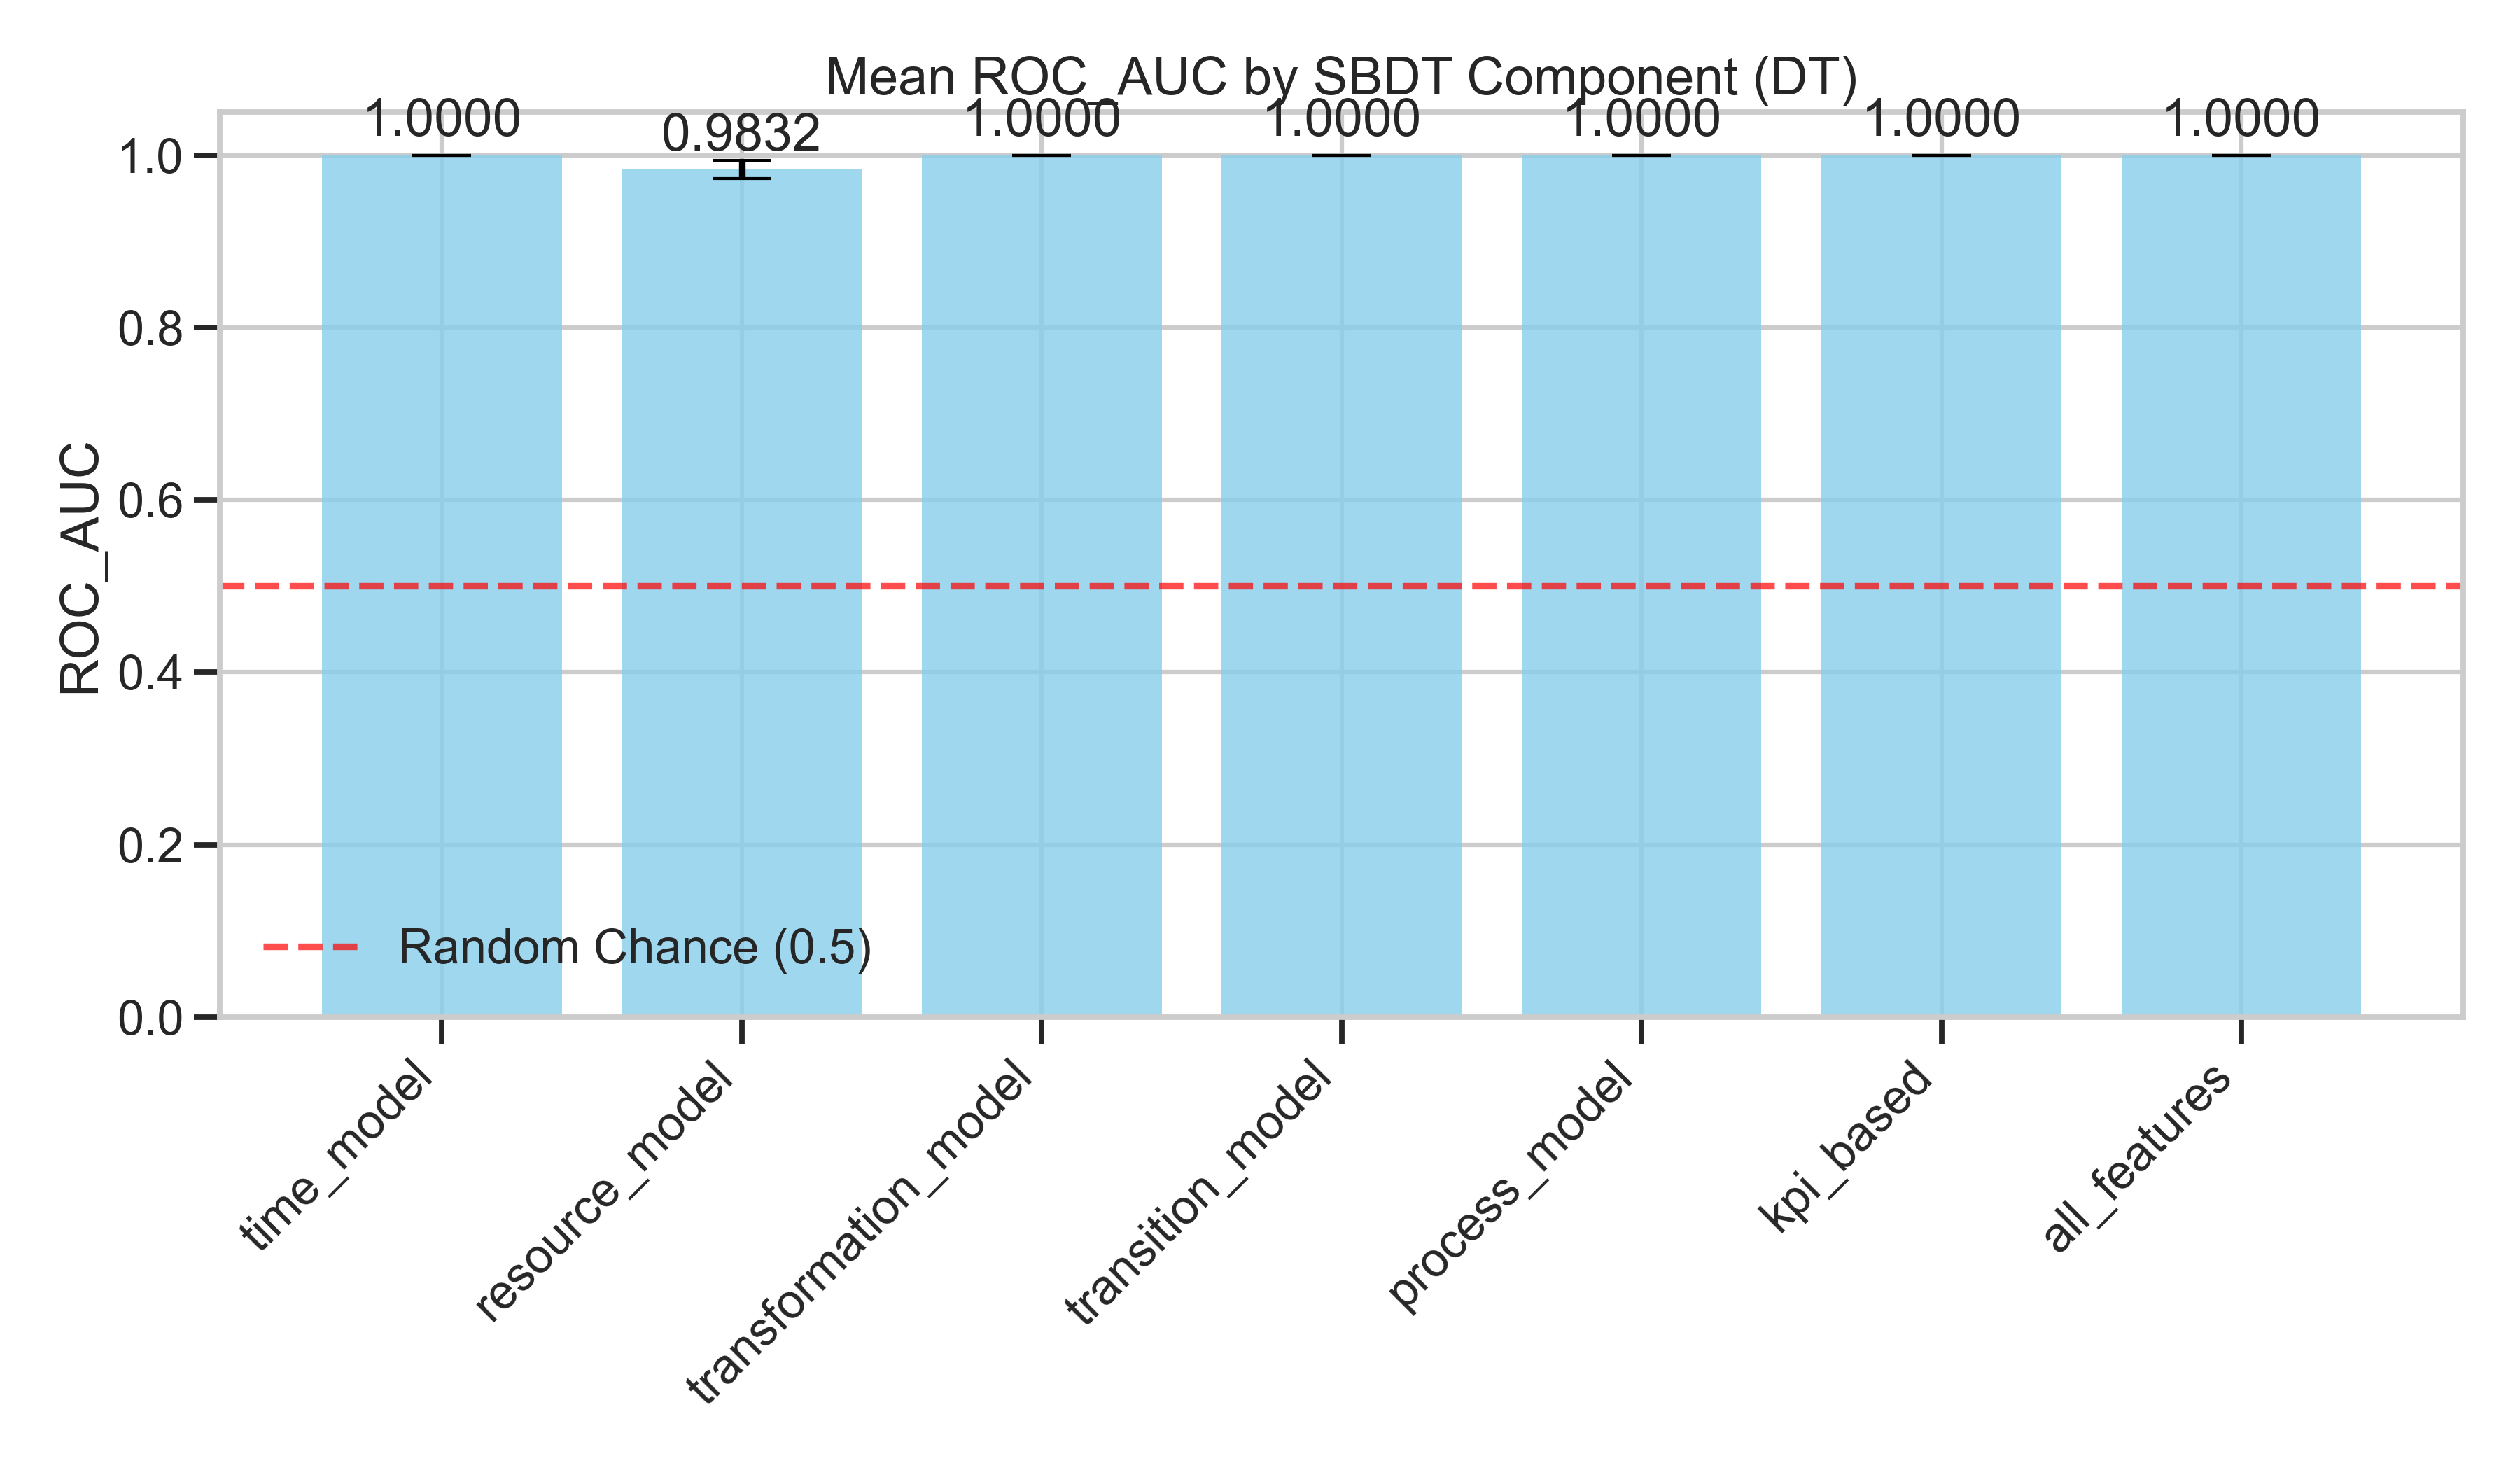
\includegraphics[width=0.8\textwidth]{figures/dt-roc-auc-by-component.png}
  \caption[Results Decision Tree]{Mean ROC AUC scores achieved by the DTree classifier when distinguishing between real and simulated data, using feature subsets corresponding to different SBDT components. Scores averaged over 10 runs. The dashed red line indicates random chance (AUC = 0.5).}
  \label{fig:dt-roc-auc}
  \caption*{Source: Own illustration.}
\end{figure}

The results from the whitebox model are highly significant. For almost all feature subsets, the DTree achieved a perfect mean ROC AUC of 1.0000, with the exception of the \texttt{resource\_model} subset which scored slightly lower but still extremely high ($\bar{S}_{obs}=0.9832 \pm 0.0104$). Correspondingly, the mean p-values were effectively zero ($< 0.0001$, reported as 0.0000) and the rejection rate was 1.00 for all components across all 10 runs. This indicates that the DTree could easily and consistently distinguish the simulated data from the real data based on the features associated with every tested SBDT component. According to the interpretation framework, this implies that, from the perspective of the whitebox model, all tested SBDT components were learned inaccurately.
Given that the mean p-value for every feature subset is far below the significance level ($\bar{p} \approx 0.0000 < \alpha = 0.05$), and the rejection rate $RR$ is 1.00 for all components, it rejects the null hypothesis ($H_0$) for every tested SBDT component based on the DTree. This provides statistically significant evidence that the model can reliably distinguish between the real process data and the simulated data using the features associated with the time model, resource model, transformation model, transition model, process model, and KPI-based perspectives, as well as when using all features combined.

\textbf{The conclusion drawn solely from this whitebox analysis is therefore that the SBDT exhibits detectable discrepancies compared to the real system across all evaluated aspects. Consequently, based on the stringent criteria of the Decision Tree's ability to find differentiating patterns (even limited to $max_depth=5$), all tested components of the SBDT are deemed inaccurate.} This suggests that, at the level of detail captured by the engineered features and marked by the DTree model, the simulation does not adequately replicate the observed behaviour of the real IoT factory. The analysis with the blackbox model in the next section will explore whether a more complex model reaches similar conclusions.

\subsection*{Results of Blackbox Model}

The blackbox validation employed the BiLSTM-based classifier described earlier in the thesis. Training this model is computationally more intensive than the DTree. Therefore, while the number of permutations ($N=1000$) and runs ($n_{runs}=10$) were maintained, the label shuffling for generating the null distribution was performed only on the test set labels for efficiency, comparing against the fixed predictions of the trained model. Furthermore, a stricter significance level of $\alpha = 0.01$ was chosen for this analysis. GPU acceleration via CUDA \autocite{NVIDIA_CUDA} was utilized to manage the computational cost.

The aggregated results from the blackbox models permutation tests are summarized in \autoref{tab:results-blackbox}, based on the report generated by the testing script. The mean AUC scores are visualized in \autoref{fig:bilstm-roc-auc}.

\begin{table}[htbp]
  \centering
  \caption[Results BiLSTM]{Blackbox BiLSTM validation results across 10 runs (N=1000, $\alpha=0.01$).}
  \label{tab:results-blackbox}
  \begin{tabular}{l l l l l p{3cm}}
    \toprule
    \textbf{Component ($\mathcal{F}_c$)} & \textbf{$\overline{\text{ROC AUC}}$} & \textbf{$\sigma_{\text{ROC AUC}}$} & \textbf{$\bar{p}$-value} & \textbf{RR} & \textbf{Assessment} \\
    \midrule
    \texttt{time\_model}                 & 0.9998                               & 0.0005                             & 0.0000                   & 1.00        & INACCURATE          \\
    \texttt{resource\_model}             & 0.9087                               & 0.1618                             & 0.0492                   & 0.90        & INACCURATE          \\
    \texttt{transformation\_model}       & 0.8705                               & 0.2094                             & 0.1879                   & 0.80        & INACCURATE          \\
    \texttt{transition\_model}           & 1.0000                               & 0.0000                             & 0.0000                   & 1.00        & INACCURATE          \\
    \texttt{process\_model}              & 0.9788                               & 0.0635                             & 0.0000                   & 1.00        & INACCURATE          \\
    \texttt{kpi\_based}                  & 0.9989                               & 0.0019                             & 0.0000                   & 1.00        & INACCURATE          \\
    \texttt{all\_features}               & 1.0000                               & 0.0000                             & 0.0000                   & 1.00        & INACCURATE          \\
    \bottomrule
  \end{tabular}
  \caption*{Source: Own tabulation.}
\end{table}

\begin{figure}[htbp]
  \centering
  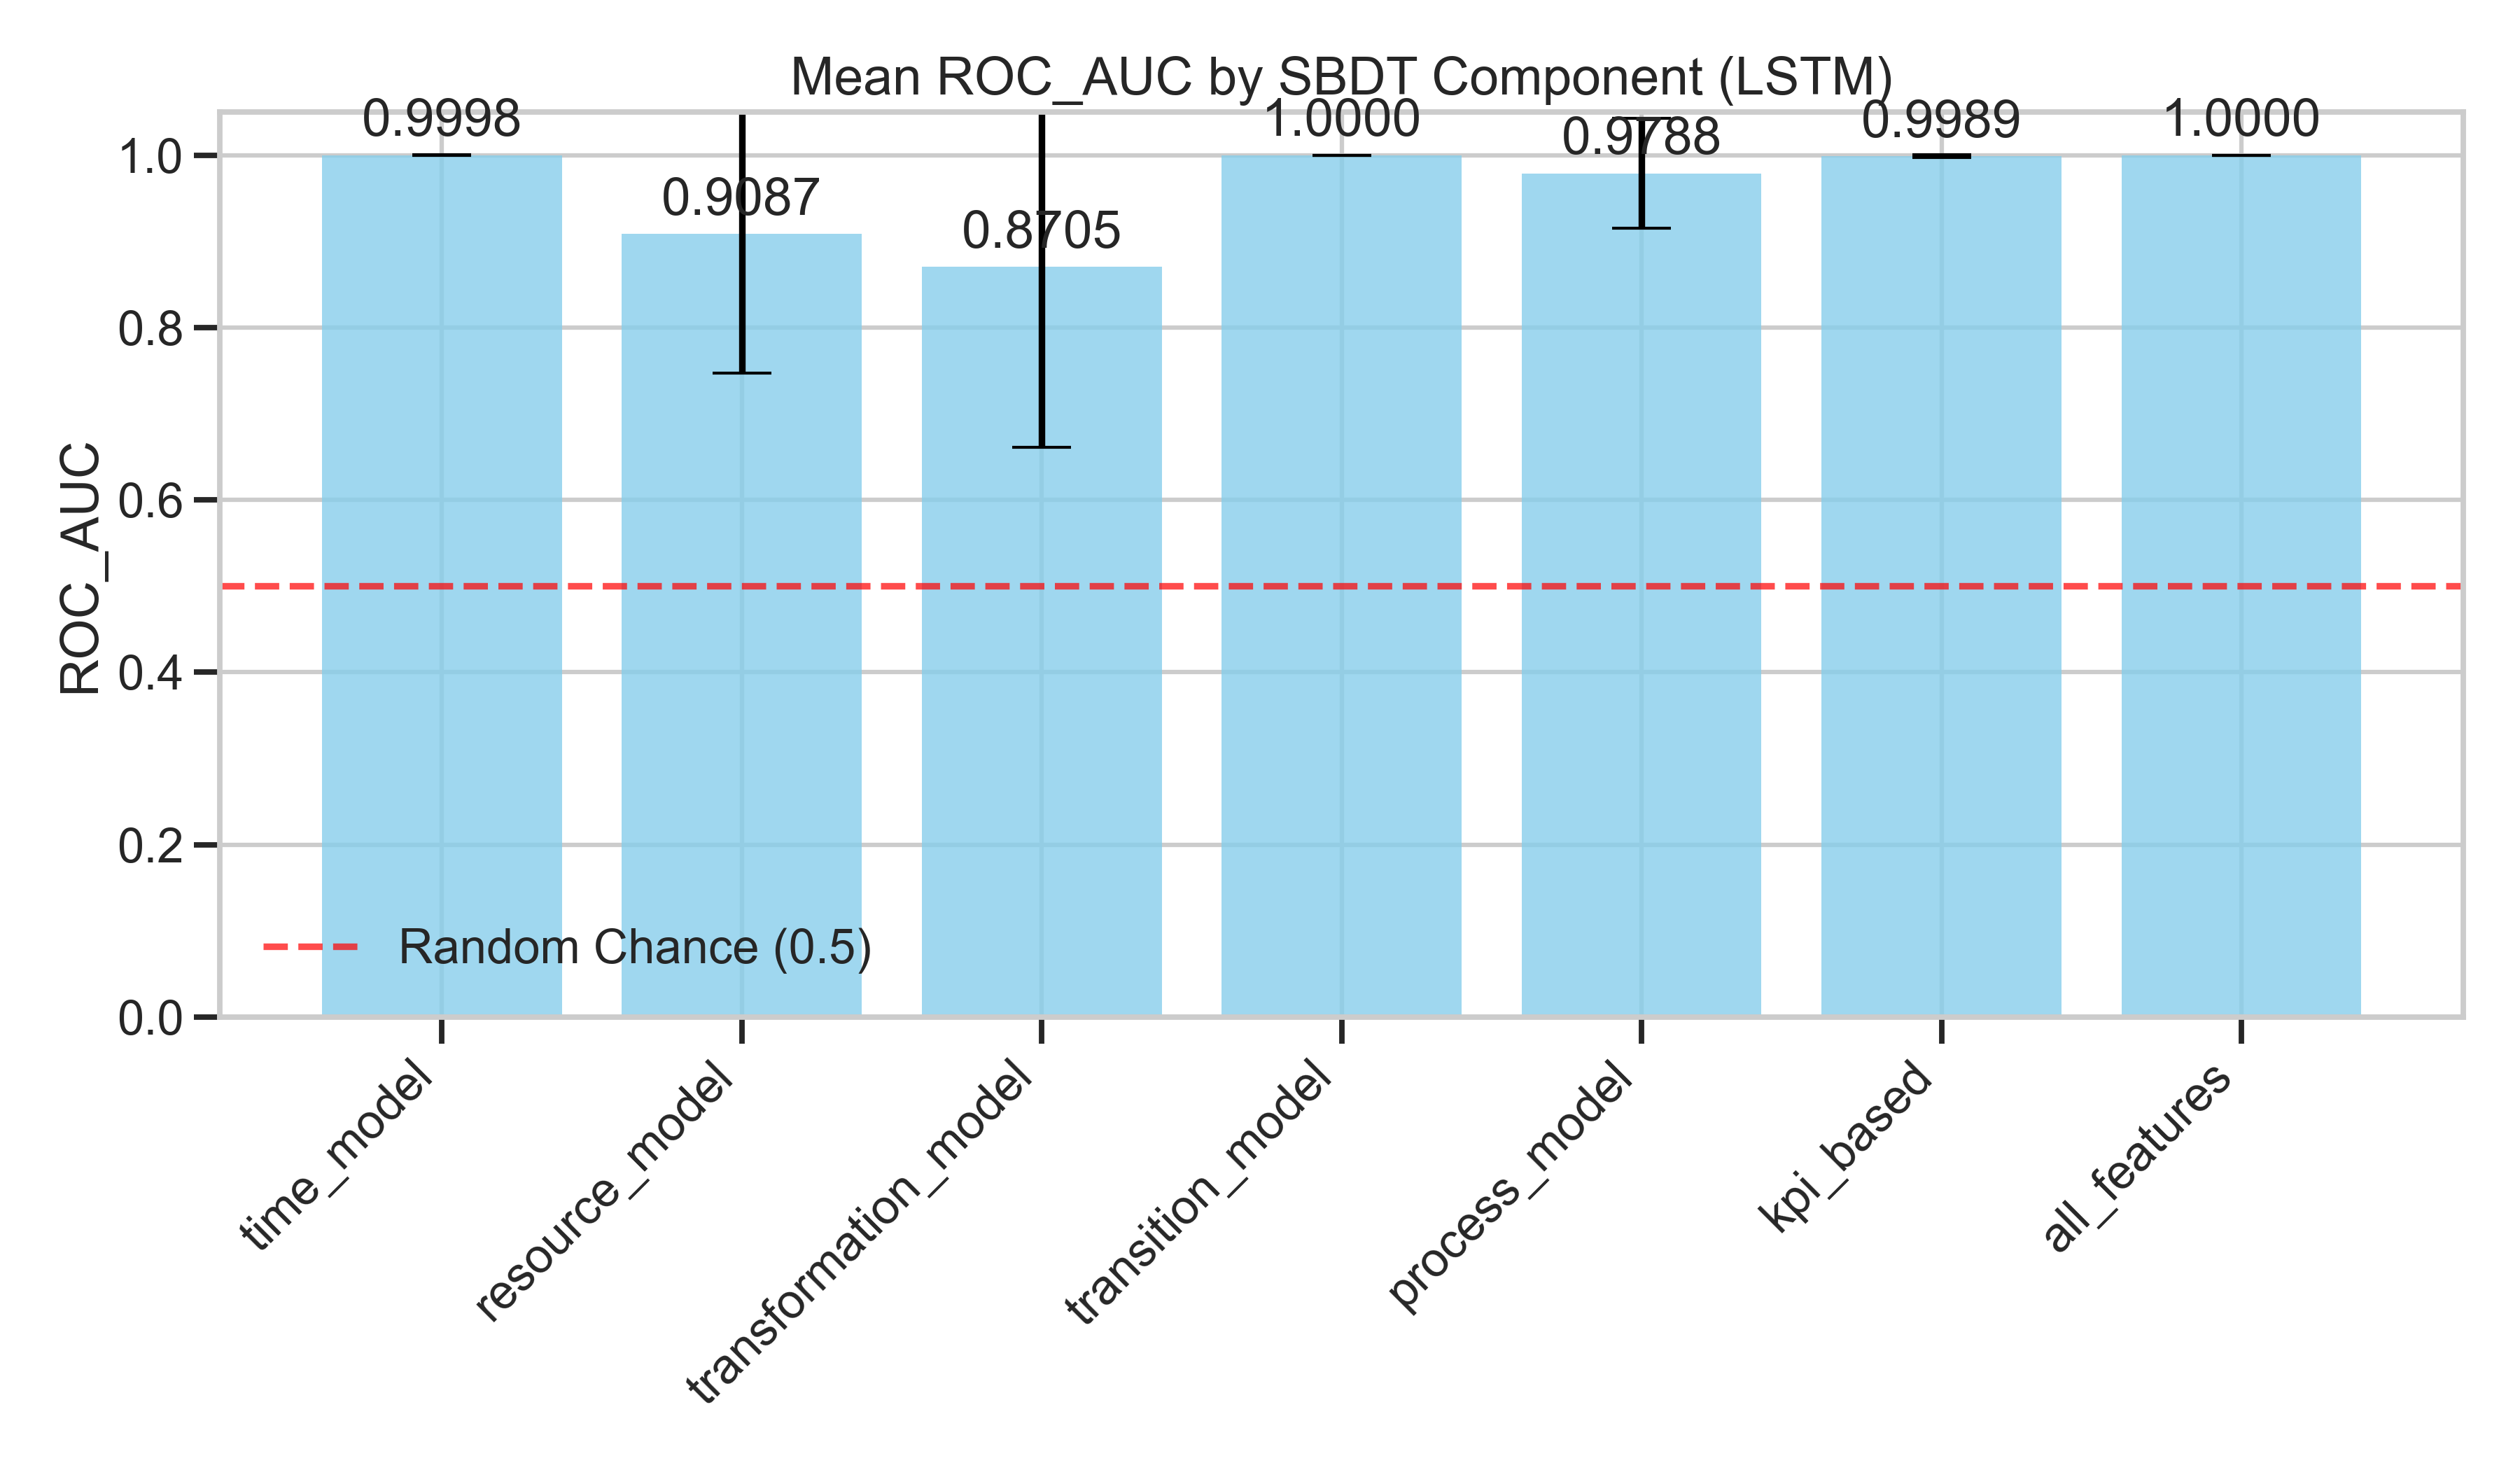
\includegraphics[width=0.8\textwidth]{figures/lstm-roc-auc-by-component.png}
  \caption[Results Blackbox model]{Mean ROC AUC scores achieved by the classifier when distinguishing between real and simulated data, using feature subsets corresponding to different SBDT components. Scores averaged over 10 runs. The dashed red line indicates random chance (AUC = 0.5).}
  \label{fig:bilstm-roc-auc}
  \caption*{Source: Own illustration.}
\end{figure}

The blackbox model results largely align with the whitebox findings, indicating significant discrepancies between the simulated and real data across various SBDT components. The BiLSTM classifier achieved very high mean ROC AUC scores for most feature subsets, particularly for \texttt{time\_model} (0.9998), \texttt{transition\_model} (1.0000), \texttt{process\_model} (0.9788), \texttt{kpi\_based} (0.9989), and \texttt{all\_features} (1.0000). For these components, the mean p-values were effectively zero, and the rejection rate $RR$ was 1.00, strongly indicating rejection of the null hypothesis ($H_0$) at the $\alpha = 0.01$ significance level.

For the \texttt{resource\_model} and \texttt{transformation\_model}, the mean ROC AUC scores were lower ($\bar{S}_{obs}=0.9087$ and $0.8705$, respectively) and exhibited considerably higher standard deviations ($\sigma_{S_{obs}}=0.1618$ and $0.2094$), suggesting greater variability in the models ability to distinguish data based on these features across the 10 runs. \textbf{Notably, while the \textit{mean} p-values (0.0492 and 0.1879) across the 10 runs were above the strict $\alpha=0.01$ threshold for these two components, $RR$ (showing the consistency of rejecting $H_0$ in individual runs) was considered the more decisive metric for the overall assessment in this multi-run framework.} The $RR$ values remained very high ($RR=0.90$ for \texttt{resource\_model}, $RR=0.80$ for \texttt{transformation\_model}). \textbf{Crucially,} a rejection rate of $0.90$ means that in 9 out of the 10 independent runs, the calculated p-value was less than the strict $\alpha=0.01$, leading to the rejection of $H_0$. Similarly, for the transformation model, $H_0$ was rejected in 8 out of 10 runs. \textbf{Therefore,} the high rejection rates across multiple runs provide strong \textbf{statistical evidence} that the BiLSTM could consistently distinguish the data \textbf{for these components as well}, supporting the rejection of $H_0$ \textbf{based on repeated testing, even considering the variability observed and the average p-value.}

\textbf{Consequently, prioritizing $RR$ which reflects statistical significance across the majority of independent runs over the potentially variable average p-value}, the analysis concludes that the blackbox model finds statistically significant differences between the real and simulated data for all tested aspects.

Similar to the whitebox analysis, the conclusion drawn from the blackbox model is \textbf{that the SBDT exhibits detectable inaccuracies compared to the real system across all evaluated components. The combination of high ROC AUC scores and, critically, the high rejection rates (RR $\ge$ 0.80 for all components) under permutation testing provide robust evidence against the null hypothesis ($H_0$) for every component. Consequently, based on the BiLSTM classifier's consistent ability to distinguish the data across multiple runs, all tested components of the SBDT are assessed as inaccurate.} This supports the finding that the current SBDT configuration, as evaluated through the engineered features, does not sufficiently replicate the behavior observed in the real IoT factory dataset.

\section{Sanity Check}
\label{sec:sanity-check}

Given the high, near-perfect ROC AUC scores observed in the main experiments (\autoref{tab:results-whitebox}, \autoref{tab:results-blackbox}), this control experiment was performed to rule out the possibility that these scores resulted from data artifacts rather than genuine SBDT fidelity issues. This 'Identical Data Control Experiment" tests if classifiers can distinguish between identical datasets solely based on assigned labels ($y=1$ versus $y=0$), using the same methodology as the main experiments but on duplicated real and simulated data separately \autocite{adebayo2018sanity}.

The results are summarized in \autoref{tab:sanity-check-results}.

\begin{table}[htbp]
  \centering
  \caption[Sanity Check]{Results of Identical Data Control Experiments (Mean ROC AUC over 10 runs)}
  \label{tab:sanity-check-results}
  \resizebox{\textwidth}{!}{%
    \begin{tabular}{l l c c c c}
      \toprule
      \textbf{Classifier} & \textbf{Feature Set ($\mathcal{F}_c$)} & \textbf{Original AUC}   & \textbf{Identical Real Data AUC} & \textbf{Identical Simulated Data AUC} & \textbf{Expected AUC}    \\
                          &                                        & \textbf{(Real vs. Sim)} & \textbf{(Real vs. Real-Copy)}    & \textbf{(Sim vs. Sim-Copy)}           & \textbf{(Random Chance)} \\
      \midrule
      Decision Tree       & \texttt{time\_model}                   & 1.0000                  & 0.3302                           & 0.3545                                & $\approx 0.5$            \\
      Decision Tree       & \texttt{resource\_model}               & 0.9832                  & 0.3916                           & 0.4140                                & $\approx 0.5$            \\
      Decision Tree       & \texttt{transformation\_model}         & 1.0000                  & 0.3903                           & 0.4072                                & $\approx 0.5$            \\
      Decision Tree       & \texttt{transition\_model}             & 1.0000                  & 0.3389                           & 0.4079                                & $\approx 0.5$            \\
      Decision Tree       & \texttt{process\_model}                & 1.0000                  & 0.3279                           & 0.4107                                & $\approx 0.5$            \\
      Decision Tree       & \texttt{kpi\_based}                    & 1.0000                  & 0.3278                           & 0.3788                                & $\approx 0.5$            \\
      Decision Tree       & \texttt{all\_features}                 & 1.0000                  & 0.3471                           & 0.3763                                & $\approx 0.5$            \\
      \midrule
      BiLSTM              & \texttt{time\_model}                   & 0.9998                  & 0.4992                           & 0.5008                                & $\approx 0.5$            \\
      BiLSTM              & \texttt{resource\_model}               & 0.9087                  & 0.4989                           & 0.5003                                & $\approx 0.5$            \\
      BiLSTM              & \texttt{transformation\_model}         & 0.8705                  & 0.5015                           & 0.4980                                & $\approx 0.5$            \\
      BiLSTM              & \texttt{transition\_model}             & 1.0000                  & 0.4998                           & 0.5007                                & $\approx 0.5$            \\
      BiLSTM              & \texttt{process\_model}                & 0.9788                  & 0.4752                           & 0.4977                                & $\approx 0.5$            \\
      BiLSTM              & \texttt{kpi\_based}                    & 0.9989                  & 0.4938                           & 0.5027                                & $\approx 0.5$            \\
      BiLSTM              & \texttt{all\_features}                 & 1.0000                  & 0.5000                           & 0.5000                                & $\approx 0.5$            \\
      \bottomrule
    \end{tabular}%
  }
  \caption*{Source: Own tabulation, incorporating results from provided summary and \autoref{tab:results-whitebox}, \autoref{tab:results-blackbox}.}
\end{table}

As shown, both classifiers achieved ROC AUC scores near the random chance baseline of 0.5 when tested on identical data in contrast to the near-perfect scores achieved on the original real vs. simulated data comparison.
This successful outcome strongly suggests the original high AUC scores were not primarily driven by artifacts. It validates the framework's core interpretation: the classifiers detected genuine, statistically significant differences between the real and simulated data. Therefore, the high AUC and RR values reported in \autoref{tab:results-whitebox} and \autoref{tab:results-blackbox} can be confidently interpreted as indicators of lower fidelity in the corresponding SBDT components, providing a reliable basis for identifying areas for model improvement.

To conclude, this chapter empirically validated the proposed VVUQ framework using the IoT Factory case study (\autoref{sec:factory}, \autoref{sec:automated-digital-twin}). The machine learning-based approach, employing both Decision Tree and BiLSTM classifiers with permutation testing (\autoref{sec:model-logic}), successfully identified statistically significant discrepancies between the SBDT and real-world data across all tested components (\autoref{tab:results-whitebox}, \autoref{tab:results-blackbox}). Crucially, identical data control experiments (\autoref{sec:sanity-check}) confirmed these findings were not due to artifacts (\autoref{tab:sanity-check-results}). The validation demonstrated the frameworks effectiveness in automatically assessing SBDT fidelity and providing component-specific feedback for improvement.